\documentclass{article}

\usepackage{graphicx}
\usepackage{tikz}
\usepackage{tikzsymbols}
\usetikzlibrary{calc,patterns,shapes.geometric}
\pagestyle{empty}
\usepackage[margin=0pt]{geometry}
\geometry{papersize={14in,12in}}

\def\centerarc[#1](#2)(#3:#4:#5){\draw[#1] ($(#2)+({#5*cos(#3)},{#5*sin(#3)})$) arc (#3:#4:#5);}

\begin{document}
	\begin{figure}
		\centering
		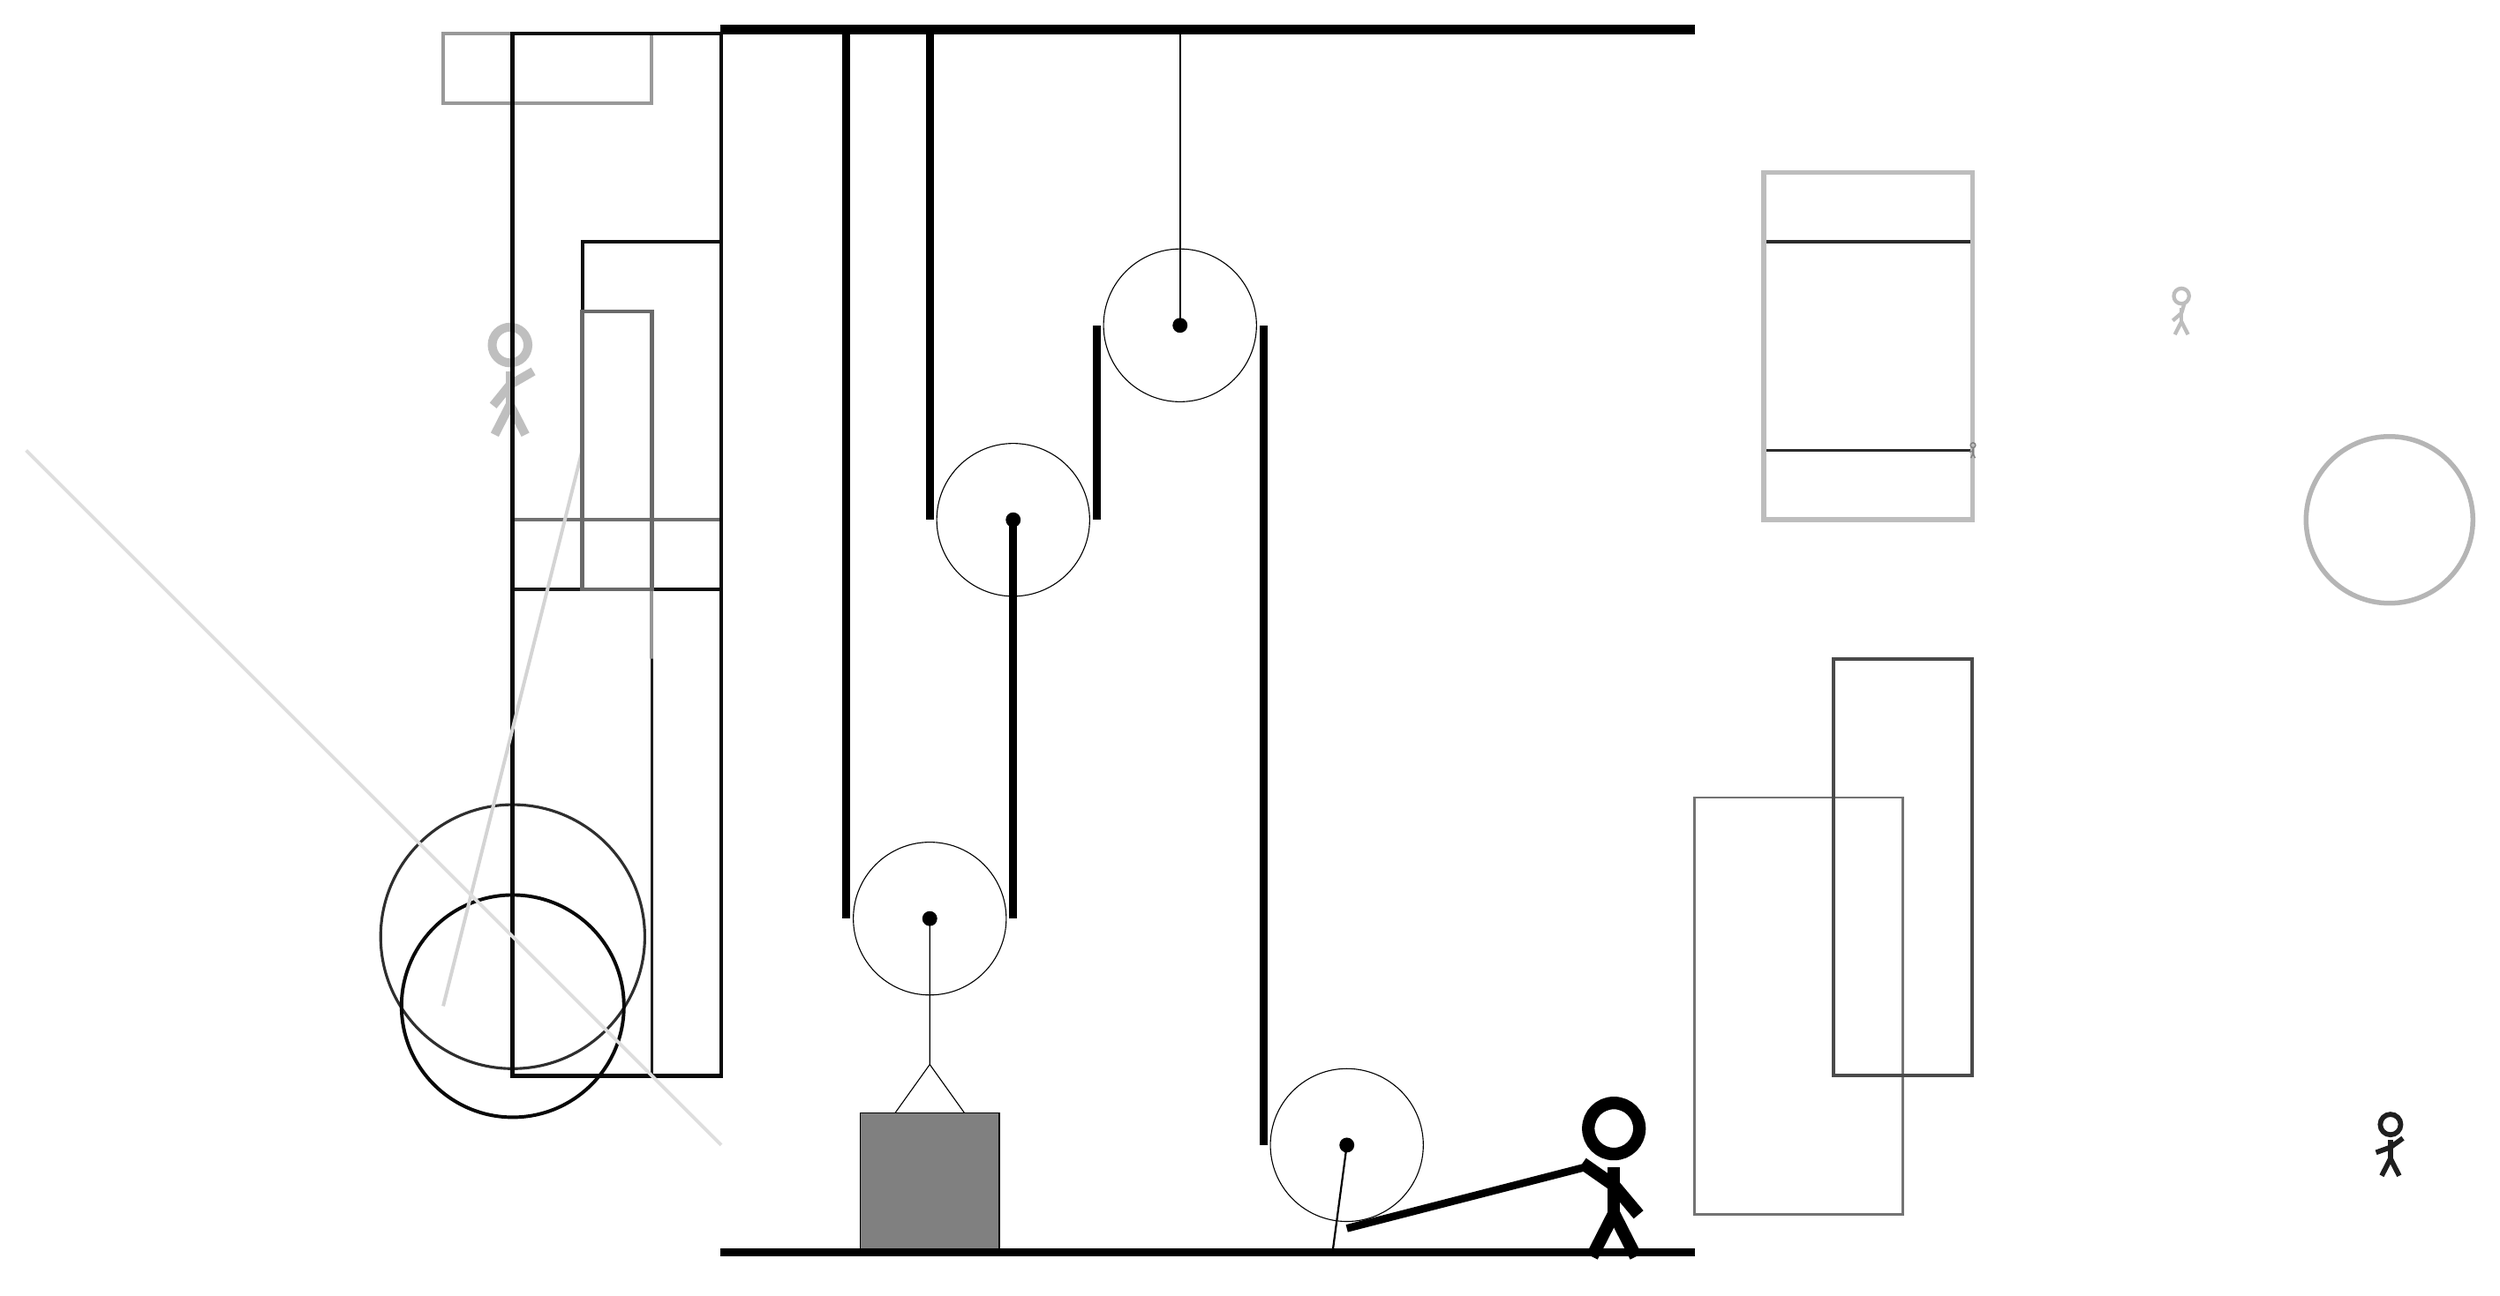
\begin{tikzpicture}
			%%%%% START %%%%%
			
			\draw[fill=black] (-2, 14) rectangle (12, 14.125);
			
			\draw (1, 1.26) circle (1.1);
			\draw[fill=black] (1, 1.26) circle (0.1);
			
			\draw (2.2, 7.0) circle (1.1);
			\draw[fill=black] (2.2, 7.0) circle (0.1);
			
			\draw (4.6, 9.8) circle (1.1);
			\draw[fill=black] (4.6, 9.8) circle (0.1);
			\draw[thick] (4.6, 9.8) -- (4.6, 14);
			
			\draw[line width=0.5mm, color=black!83] (13, 11) rectangle (16, 8);
			
			\node[line width=0.3mm, color=black!26] at (19, 10) {\Strichmaxerl[3][41][73]};
			\draw[line width=0.7mm, color=black!26] (13, 7) rectangle (16, 12);
			\node[line width=0.4mm, color=black!88] at (22, -2) {\Strichmaxerl[4][20][36]};
			\draw[line width=0.3mm, color=black!55] (12, -3) rectangle (15, 3);
			\node[line width=0.6mm, color=black!50] at (16, 8) {\Strichmaxerl[1][15][86]};
			
			\draw[line width=0.5mm, color=black!40] (-3, 14) rectangle (-6, 13);
			\draw[line width=0.5mm, color=black!71] (14, 5) rectangle (16, -1);
			\draw[line width=0.4mm, color=black!89] (-3, 6) rectangle (-5, -1);
			
			\draw[line width=0.5mm, color=black!56] (-2, 7) rectangle (-5, -1);
			
			\node[line width=0.2mm, color=black!25] at (-5, 9) {\Strichmaxerl[7][51][30]};
			
			\draw[line width=0.5mm, color=black!15](-5, -1) -- (-5, 5);
			\draw [line width=0.4mm, color=black!82](-5, 1) circle (1.9);
			
			\draw[line width=0.6mm, color=black!96] (-2, -1) rectangle (-5, 14);
			\draw [line width=0.5mm, color=black!97](-5, 0) circle (1.6);
			\draw[line width=0.5mm, color=black!95] (-4, 6) rectangle (-2, 11);
			
			\draw[line width=0.5mm, color=black!41] (-3, 5) rectangle (-3, 8);
			\draw[line width=0.5mm, color=black!17](-6, 0) -- (-4, 8);
			\draw [line width=0.7mm, color=black!29](22, 7) circle (1.2);
			
			\draw[line width=0.5mm, color=black!13](-2, -2) -- (-12, 8);
			\draw[line width=0.6mm, color=black!59] (-4, 10) rectangle (-3, 6);
			
			
			\draw (7.0, -2) circle (1.1);
			\draw[fill=black] (7.0, -2) circle (0.1);
			\draw[thick] (7.0, -2) -- (6.8, -3.5);
			
			\draw (1, 1.26) -- (1, -0.84) -- (0.5, -1.54) -- (1.5, -1.54) -- (1, -0.84);
			\draw[fill=black!50] (0, -1.54) rectangle (2, -3.54);
			\draw[line width=1.1mm] (-0.2, 14) -- (-0.2, 1.26);
			\centerarc[line width=1.1mm](1, 1.26)(180:360:1.2000000000000002);
			\draw[line width=1.1mm](2.2, 1.26) -- (2.2, 7.0);
			\draw[line width=1.1mm] (1.0, 14) -- (1.0, 7.0);
			\centerarc[line width=1.1mm](2.2, 7.0)(180:360:1.2000000000000002);
			\draw[line width=1.1mm](3.4, 7.0) -- (3.4, 9.8);
			\centerarc[line width=1.1mm](4.6, 9.8)(0:180:1.2000000000000002);
			\draw[line width=1.1mm] (5.8, 9.8) -- (5.8, -2);
			\centerarc[line width=1.1mm](7.0, -2)(0:90:-1.2000000000000002);
			\draw[line width=1.1mm](7.0, -3.2) -- (10.5, -2.3);
			
			\node at (10.8, -2.5) {\Strichmaxerl[10][-35][-50]};
			
			\draw[fill=black] (-2, -3.5) rectangle (12, -3.6);
			
			%%%%% END %%%%%
		\end{tikzpicture}
	\end{figure}	
\end{document}